\casesection{Channel with curvilinear grid distortion\label{case:griddistortion}}


\paragraph*{Purpose}
The purpose of this validation study is to investigate the effect of a misaligned grid, i.e.\ a grid that makes an angle with the flow direction, on the accuracy of the model results. This validation study is directly derived from the validation document for Delft3D.


\paragraph*{Linked claims}
Claims that are related to the current test case are:
\begin{itemize}
\item \clrefnoh{cl:generalGrids}
\end{itemize}


\paragraph*{Approach}
A uniform flow in a simple straight channel over a sloping topography is considered. In the steady state, the slope of the water level should equal the slope of the bed. In this test case, it is examined to what extent the numerical solution is dependent on the grid it is computed on. For this purpose, the outcomes obtained on a Cartesian grid are compared with the outcomes obtained on a sinusoidally distorted grid. This sinusoidally distorted grid is shown in \Fref{fig:distortedgrid}. A computation on an equivalent, strictly Cartesian grid of $M \times N = 10 \times 80$ cells is carried out for comparison.

\begin{figure}[h!]
\begin{center}
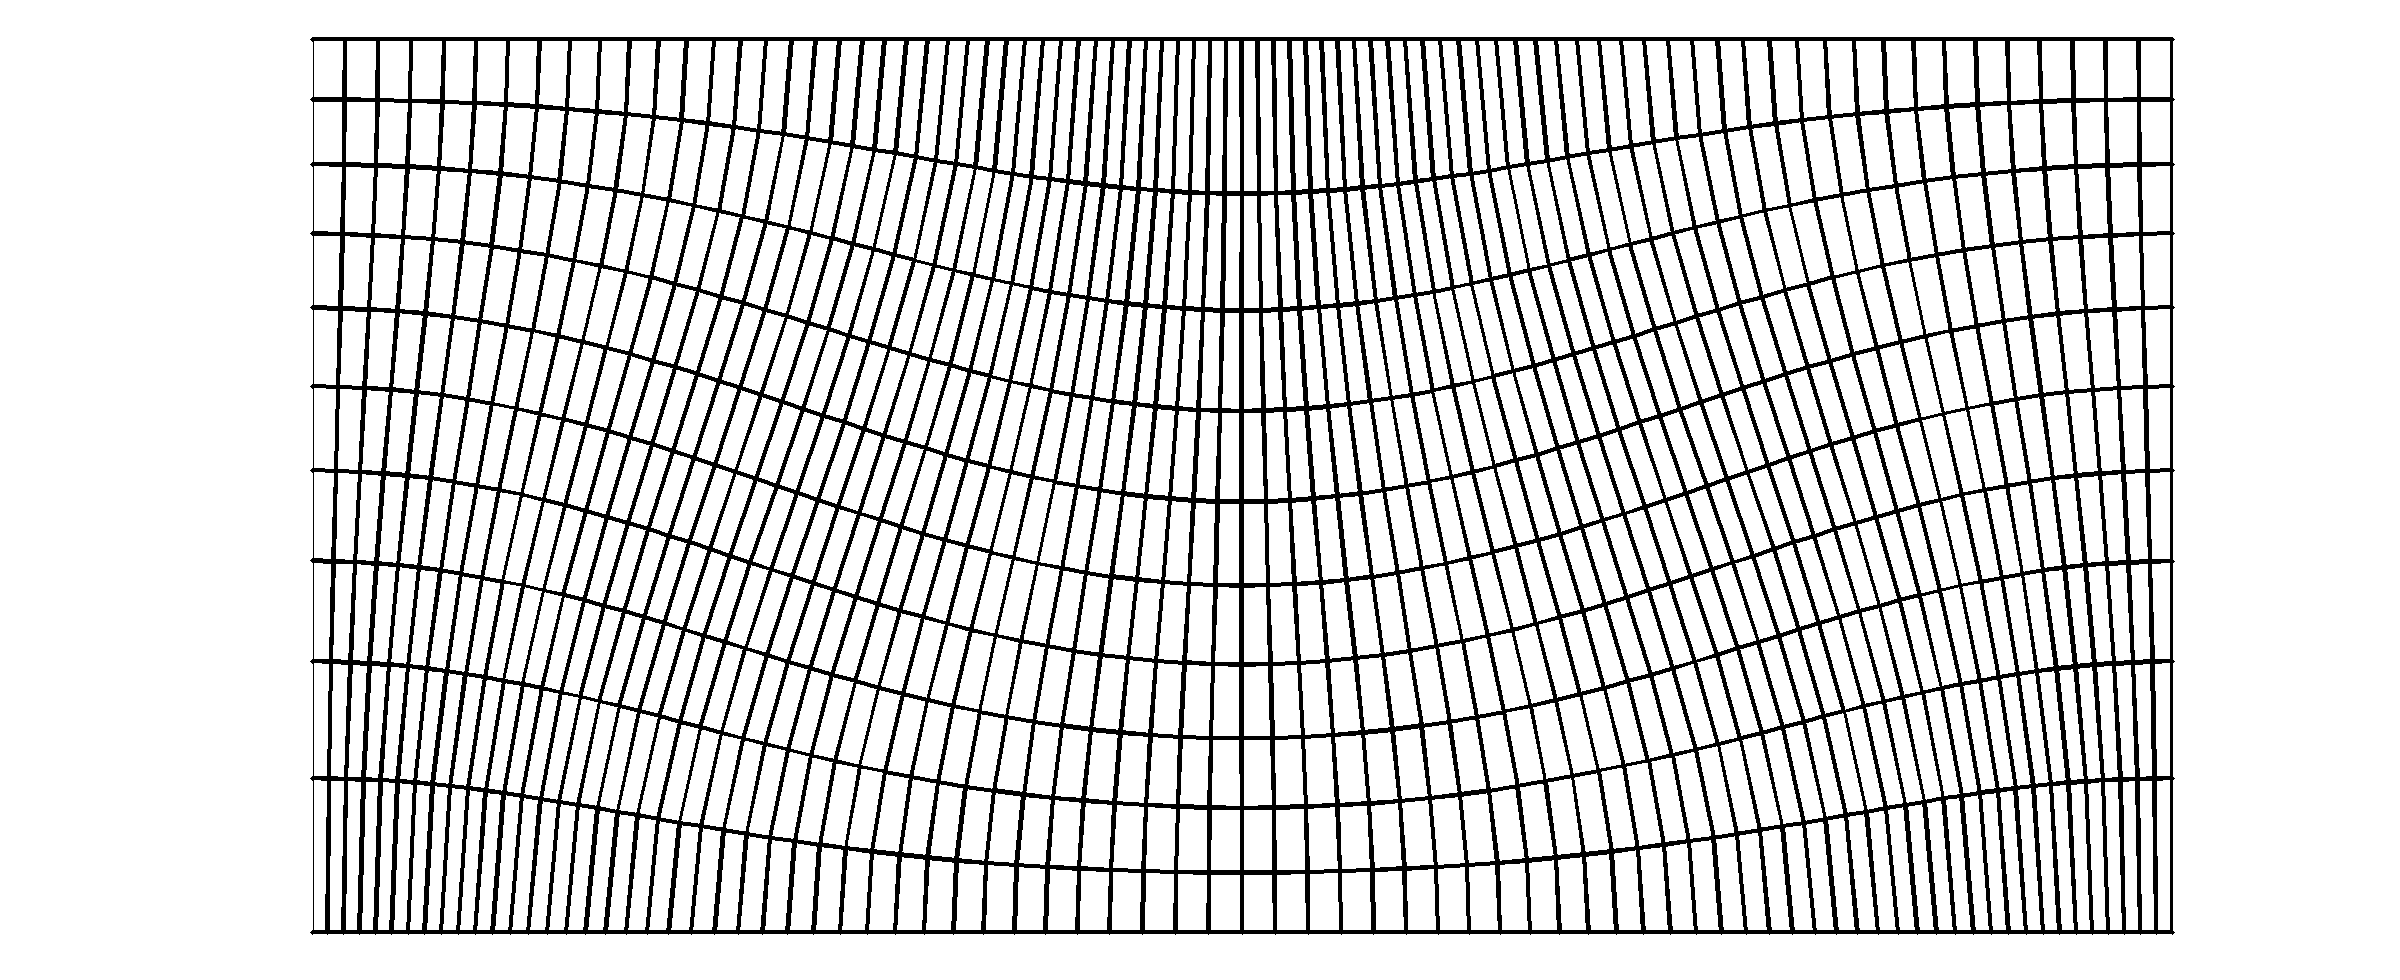
\includegraphics[width=0.5\columnwidth]{figures/distortedgrid.png}
\end{center}\caption{The computational grid for curvilinearly distorted grid case. The bed level ranges from -4 m (left) to -4.5 m (right) w.r.t.\ the reference level. The flow is from left to right. \label{fig:distortedgrid}}
\end{figure}

To enable academic comparison of the computational output with a known analytical solution, the slope of the bed is set varying linearly with a slope $i_b$. Given a discharge $Q$ and a friction coefficient (in this case, Ch\'ezy's factor $C$ is used), an equilibrium water depth $d_e$ can be computed as:
\begin{equation}\label{eq:equilibriumdepth}
d_e = \left(\frac{Q}{B C \sqrt{i_b}}\right)^{2/3}.
\end{equation}



\paragraph*{Model description}
The settings for the computation are (taken from the Delft3D validation document):
\begin{itemize}
\item length $L = 500$ m and width $B = 240$ m,
\item bed slope $i_b = 10^{-3}$, 
\item inflow velocity $U = 2.933654$ m/s or inflow discharge $Q = 1434.2047$ m$^3$/s, 
\item Ch\'ezy's coefficient $C =  65$ m$^{1/2}$/s.
\end{itemize}
With this parameters, the equilibrium depth is $d_e = 2.037$ m. Including the $\Delta x / 2$ distance between the outflow boundary and the cell centers of the ghost cells, the output water level is set equal to:
\begin{eqnarray*}
h_{out} &=& \textrm{bed level} + \textrm{equilibrium depth} - i_b \cdot \Delta x / 2  \\
        &=& -4.5 + 2.037 - 10^{-3} \cdot 500 / 80 / 2  \\
        &=& -2.466125~\textrm{m+NAP}
\end{eqnarray*}
Hence, the output water level is set equal to -2.466125 m w.r.t.\ the reference level.  Two specific settings to be mentioned are:
\begin{enumerate}
\item the location of the outflow water levels is set on the cell center of the ghost cell outside the grid, being mirrored due to grid staggering (i.e.\ \texttt{izbndpos = 0}),
\item at the inflow boundary, no specific corrections are made for the interpolation of the water levels, based on the downwind water level (i.e.\ \texttt{jbasqbnddownwindhs = 0}).
\end{enumerate}
The two computations are carried out twice: one time with a \textbf{velocity} boundary condition upstream, and one time with a \textbf{discharge} boundary condition upstream.


\paragraph*{Results}
\Fref{fig:distortedgridresult} shows the water depth at the end of the simulation time in case a \textbf{velocity} condition is applied at the inflow boundary. One can see that deviations from the analytical equilibrium depth are present. The closer to the outflow boundary, the more the depth approaches the analytical equilibrium depth of 2.037 m.

\begin{figure}[h!]
\begin{center}
\includegraphics[width=0.7\columnwidth]{../../c030_Curvi_griddistortion/doc/figures/distortedgridresult.png}
\end{center}\caption{The water depth at the end of the simulation time (steady state solution). Upper panel: results on the Cartesian grid; lower panel: results on the curvilinearly distorted grid. For this result, a \textbf{velocity} condition is applied at the inflow boundary. The analytical equilibrium depth is 2.037 meters. \label{fig:distortedgridresult}}
\end{figure} 

For this case with curvilinear distortion of the grid, the deviations from the analytical solution are significantly larger for the distorted grid compared to the rectangular grid. It should, moreover, be remarked that this two-dimensional case does not attain the same accuracy for this type of case as the one-dimensional case does (cf. case e02-f05-c020).


\Fref{fig:distortedgridresultdischarge} shows the water depth at the end of the simulation time in case a \textbf{discharge} condition is applied at the inflow boundary.

\begin{figure}[h!]
\begin{center}
\includegraphics[width=0.7\columnwidth]{../../c031_Curvi_griddistortion_discharge/doc/figures/distortedgridresult.png}
\end{center}\caption{The water depth at the end of the simulation time (steady state solution). Upper panel: results on the Cartesian grid; lower panel: results on the curvilinearly distorted grid. For this result, a \textbf{discharge} condition is applied at the inflow boundary. The analytical equilibrium depth is 2.037 meters. \label{fig:distortedgridresultdischarge}}
\end{figure} 

As \Fref{fig:distortedgridresultdischarge} shows, the deviations in the outflow region are quite comparable with their equivalents from \Fref{fig:distortedgridresult}. However, it is seen that the deviations become smaller the more the inflow boundary is approached. From this it could be concluded that the discharge inflow boundary condition is favorable over the velocity inflow boundary condition.

Remark that the timestep $\Delta t$ is computed automatically, based on a CFL limit value of 0.7. If \texttt{jbasqbnddownwindhs = 1} is chosen in the mdu-file, the computation on the curvilinearly distorted grid starts wiggling.


\paragraph*{Conclusions}
Misalignment of the grid has a clear effect on the accuracy of the model results. For the curvilinearly distorted grid, the maximum deviation from the analytical solution for the equilibrium depth is significantly larger compared to the equivalent Cartesian grid case.


\paragraph*{Version}
This test has been carried out with version dflow-fm-x64-1.1.116.36629.